\documentclass{standalone}
\usepackage{tkz-fct}
\usepackage{tkz-euclide}
\usepackage{color}
\renewcommand*\familydefault{\sfdefault}
\usepackage{sansmath}
\sansmath
\definecolor{gray75}{gray}{0.75}
\begin{document}
 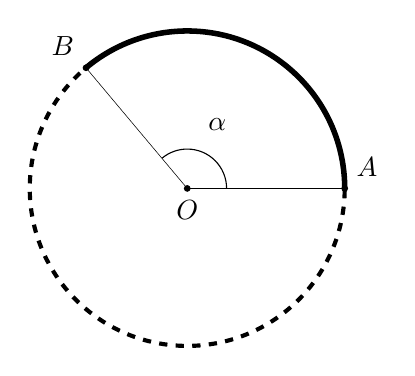
\begin{tikzpicture}[scale=2]

   \tkzDefPoints{0/0/O,1/0/A}
   \tkzDrawCircle[color=black, dashed, line width=1.5pt](O,A)
   \tkzDefPointBy[rotation= center O angle 130](A)
   \tkzGetPoint{B}
   \tkzDrawSegment(O,A)
   \tkzDrawSegment(O,B)
   \tkzDrawArc[color=black,line width=2pt](O,A)(B)
   \tkzDrawPoints(A,B,O)
   \tkzLabelPoints[above right](A)
      \tkzLabelPoints[above left](B)

   \tkzLabelPoints[below](O)

   \tkzPicAngle["$\alpha$",draw=black,
-,angle eccentricity=1.8,
angle radius=0.5cm](A,O,B)

\end{tikzpicture}
\end{document}
